\documentclass[10pt,a4paper]{article}
\usepackage[T1]{fontenc}
\usepackage[a4paper]{geometry}
\usepackage{xcolor}
\usepackage{amssymb}
\usepackage{amsmath}
\usepackage{graphicx}
\usepackage{tabularx}
\usepackage{multirow}
\usepackage{subfigure}
\usepackage{verbatim}
\usepackage{fancyhdr}
\usepackage{listings}
\usepackage{../common/espacs}

\title{Esercitazione 2}
\date{October 12, 2012}

\pagestyle{fancy}
\headheight 35pt

\begin{document}
\lstset{language=[ISO]C++}
\maketitle

Let $f \in C^{1} \left( a, b \right)$ be a real function that goes to zero at
the point $\alpha\in (a, b)$. A robust algorithm to find a zero of such a
function can be built joining a low order method, for which global convergence
is guaranteed, with a high order method. The high order method reaches the
zero with a lower number of steps with respect to the low order one, but the
convergence is guaranteed only if the guess is sufficiently close to the zero.
This guess can be computed using the low order method with a coarse tolerance
rate.


%%%%%%%%%%%%%%%%%%%%%%%

\section*{Esercizio 1}

Starting from the example \texttt{QuadratureRule/baseVersion}
\begin{enumerate}
  \item extend the use of GetPot in order to pass the integrand function
  directly from the data file

  \item add a Gaussian quadrature rule, templatized on the number of quadrature
  points. The Gaussian rule should derive from the common base class
  \cpp{StandardQuadratureRule}. The points and weights can be computed using the
  \texttt{legendre\_rule} library

  \item compute the integral of the function
    \begin{align*}
    f(x) = e^x x
    \end{align*}
  in $[0,1]$ using all the available quadrature rules.

  \item implement a MonteCarlo quadrature rule, that also derives from
  \cpp{QuadratureRule}.
\end{enumerate}


\section*{Solutions}

\begin{enumerate}

    \item In order to make the code reusable, we choose to group all the
    interfaces for the classes in a header file, while the implementations are
    in a corresponding source file. There is also a separate header file for
    the common definitions, such as \cpp{enum}s and \cpp{typedef}s

    \lstset{basicstyle=\scriptsize\sf}
    \lstinputlisting{./src/1/src/rootfinding.hpp}
    \lstset{basicstyle=\sf}

    In this case, the name defined by \cpp{rootfinding.hpp} are exported in the
    \cpp{Rootfinding} \cpp{namespace}.

    here follow the listings for the header file and source file that implement
    the \cpp{Bisection} and \cpp{Newton} classes.
    % Bisection
    \lstset{basicstyle=\scriptsize\sf}
    \lstinputlisting[caption=\cpp{Bisection} class interface]
      {src/1/src/bisection.hpp}
    \lstset{basicstyle=\sf}
    note that all the private attributes in the class are in the form
    \cpp{M_attributename}. This is a common approach to clearly state in the
    implementations which variables are local and which are class variables.

    The \cpp{converged} method is an \cpp{inline} function. The \cpp{inline}
    directive tells the compiler that it should try to insert the whole body of
    the function where it is called, instead of issueing a call. As it is done
    in the code, it is still possible to separate the declaration and the
    definition of the method. All the methods that are directly declared inside
    a class are treated as \cpp{inline}. If the method is instead implemented
    outside the class, it must be in a header file. It is common practice to
    insert only very short methods directly inside the class. The \cpp{inline}
    directive is available also for free functions, and it behaves in the same
    way.
    \lstset{basicstyle=\scriptsize\sf}
    \lstinputlisting[caption=\cpp{Bisection} class implementation]
    {src/1/src/bisection.cpp}
    \lstset{basicstyle=\sf}
    Inside the constructor of the class it is possible to call explicitly the
    constructors of the attributes of the class. In this case, the members 
    \cpp{M_tol}, \cpp{M_maxit} and \cpp{M_check} are initialized directly from
    the values of \cpp{tol}, \cpp{maxit} and \cpp{check}, respectively.

    The notes for the \cpp{Newton} class are analogous to the ones for the
    \cpp{Bisection} class. Here follows the listings for this class
    % Newton
    \lstset{basicstyle=\scriptsize\sf}
    \lstinputlisting[caption=\cpp{Newton} class interface]
    {src/1/src/newton.hpp}
    \lstinputlisting[caption=\cpp{Newton} class implementation]
    {src/1/src/newton.cpp}
    \lstset{basicstyle=\sf}


    \item Here follows the listings for the \cpp{Robust} class, subdivided in a
    header file and a source file.
    % Robust
    \lstset{basicstyle=\scriptsize\sf}
    \lstinputlisting[caption=\cpp{Robust} class interface]
        {src/1/src/robust.hpp}
    \lstinputlisting[caption=\cpp{Robust} class implementation]
        {src/1/src/robust.cpp}
    \lstset{basicstyle=\sf}

    inside the \cpp{Robust} class there are the definitions for the types for
    the coarse approximation of the zero (\cpp{coarseT}) and for the high order
    method used to refine the result (\cpp{fineT}). This can be useful if we
    decide to change one of the two methods with another one that uses the same
    interface. The student can try to implement as an homework a modified
    Newton method and introduce it in \cpp{Robust}. In the future we will see
    how to generalize this technique with the introduction of templates.
    The tolerance required for the coarse method is defined as the product of
    the final tolerance times the \cpp{M\_cfratio} (\emph{coarse-to-fine ratio})
    coefficient. The accessor member functions allow the access to
    non-modifiable memebers with a \cpp{const} method.

    The \cpp{Makefile} that compiles \cpp{bisection}, \cpp{newton} and
    \cpp{robust} produces a static library named \cpp{librootfinding.a}. Once
    the library is available, it can be used by other programs, such as the ones
    for \emph{Point 3}, specifying to the compiler the place (with
    \texttt{-Llib}) and the library name (with \texttt{-lrootfinding}).

    The structure for the \cpp{bisection}, \cpp{newton} and \cpp{robust} has a
    lot of common features. Replicating similar definitions is not only poor
    design, but can also lead to errors, for example if the classes must have a
    consistent interface. A better approach would be to create
    \cpp{IterativeMethod} base class from which all the other three derive.

    \item Here follows the code for the \emph{main program} for the solution of
    the third point. The implementation that it refers to is the one introduced
    in the previous points.
    \lstset{basicstyle=\scriptsize\sf}
    \lstinputlisting{./src/1/bn.hpp}
    \lstset{basicstyle=\sf}
    in this case the \cpp{Bisection}, \cpp{Newton} and \cpp{Robust} classes are
    stored in the \verb!./src/! folder.
    \lstset{basicstyle=\scriptsize\sf}
    \lstinputlisting{./src/1/bn.cpp}
    \lstset{basicstyle=\sf}

    Note in the \verb1main1 the use of two namespaces, \cpp{std} and
    \cpp{RootFinding}.

    \item Here follows the implementation for the \cpp{Robust} class. The
    overloading of \cpp{operator<<} is totally similar for the other two
    classes.
    \lstset{basicstyle=\scriptsize\sf}
    \lstinputlisting[linerange={15-29}]{./src/2/src/robust.cpp}
    \lstset{basicstyle=\sf}

    Note that the function that overloads the stream operator uses the private
    members of the class. This is the reason why it is declared as a
    \cpp{friend} function with the definition
    \lstset{basicstyle=\scriptsize\sf}
    \lstinputlisting[linerange=46-47]{./src/1.5/src/robust.hpp}
    \lstset{basicstyle=\sf}

    The code can be tested with the following \emph{main program}
    %
    \lstset{basicstyle=\scriptsize\sf}
    \lstinputlisting{./src/1.5/bn.cpp}
    \lstset{basicstyle=\sf}
    %
    and this is the corresponding \emph{output}
    \begin{verbatim}
0.707107
* Robust Method *
Tolerance           :   1e-06
Max # of iterations :   100
Convergence check   :   increment
# of iterations (C) :   3
# of iterations (F) :   4
C-to-F tol ratio    :   200000
    \end{verbatim}

\end{enumerate}


%%%%%%%%%%%%%%%%%%%%%%

\section*{Es. 2}

Keeping in mind the first exercise

\begin{enumerate}

    \item separate the program in multiple files, in a modular way, so that
    code usability is improved. Hint: group all implementations in a source
    file, add a correspondent header file and keep the main in a third file.

    \item repeat the last point of the first Ex. 1

    \item knowing that the exact solution for the previous point is
    $x=\sqrt{0.5}$, modify the code in order to save the distance between the
    current approximate solution and previous approximate solution in a file.
    Plot the solution with \texttt{gnuplot}. Comment the results using the
    theory.

\end{enumerate}

\subsection*{Exercise 2 solution}

Here follows the listing for the \emph{header file} that contains all the
declarations of the functions in the code.
% zerofun.hpp
\lstset{basicstyle=\scriptsize\sf}
    \lstinputlisting[caption=Function declarations for computing the zero of a
    function.] {src/zerofun.hpp}
\lstset{basicstyle=\sf}

We put the corresponding definitions in the \emph{source file}
\texttt{zerofun.cpp}:
\lstset{basicstyle=\scriptsize\sf}
    \lstinputlisting[caption=Function definitions for computing the zero of a
    function.] {src/zerofun.cpp}
\lstset{basicstyle=\sf}

The instruction \texttt{assert(u*f(b)<0.0);} is used to perform a simple error
checking. If the boolean instruction inside is not verified, the program stop
immediately and an error message is generated.

We have also the listing for the file \texttt{bn.cpp} that contains the main
program
\lstset{basicstyle=\scriptsize\sf}
    \lstinputlisting[caption=function definition and main program.]
    {src/bn.cpp}
\lstset{basicstyle=\sf}

The compilation can be peformed with
\begin{verbatim}
g++  -c -o bn.o bn.cpp -Wall
g++  -c -o zerofun.o zerofun.cpp -Wall
g++  -o bn bn.o zerofun.o
\end{verbatim}

The files \texttt{bn.o} and \texttt{zerofun.o} are the translation to object
code of the type and function definitions that we wrote in the corresponding
source files. The executable \texttt{bn} is created throught the \emph{linking}
of the object files together with the necessary libraries.

The \cpp{assert} can be disabled with the \cpp{-DNDEBUG} flag that must be
passed to the compiler when compiling files that contain it, i.e.
\begin{verbatim}
g++  -c -o bn.o bn.cpp -Wall
g++  -c -o zerofun.o zerofun.cpp -Wall -DNDEBUG
g++  -o bn bn.o zerofun.o
\end{verbatim}

In order to graphically see the error, it is possible to pass two additional
arguments to the functions  \texttt{bisection}, \texttt{newton} and
\texttt{robust}. The first one is the exact solution, while the second is the
name of the file for the output.
The listing for the \texttt{bng.cpp} file is as follows
\lstset{basicstyle=\scriptsize\sf}
    \lstinputlisting[caption=Function definition and main program.]
        {src/withGnuplot/bng.cpp}
\lstset{basicstyle=\sf}

we note at the end the call to the operating system that uses the file
\texttt{print\_data} with the following commands
\begin{verbatim}
set terminal png
set output "grafico.png"
plot "data" with lines
\end{verbatim}
The listing for \texttt{zerofung.hpp} is basically the same as
\texttt{zerofun.hpp}, while the listing for \texttt{zerofung.cpp} is
\lstset{basicstyle=\scriptsize\sf}
    \lstinputlisting[caption=Definitions for the functions to compute a zero of
        a function.]{src/withGnuplot/zerofung.cpp}
\lstset{basicstyle=\sf}

Note how the functions \texttt{bisection} and \texttt{newton} manage the file.
First of all it is declared, using the scope resolution operator \cpp{::} to
access the members in the \cpp{std} namespace. Afterwards it is opened in the
out mode for \texttt{bisection}, and out and app for \texttt{newton}.i This
means that in the second case the files are written at the end of the file,
without deleting any previous content. There is also a test to verify that the
file has been properly opened. The data output is performed inside the loops in
a way that is totally similar to printing to screen. at the end of each function
the file is closed.

This is the graph generated by the code
\begin{figure}[!h]
    \centering
    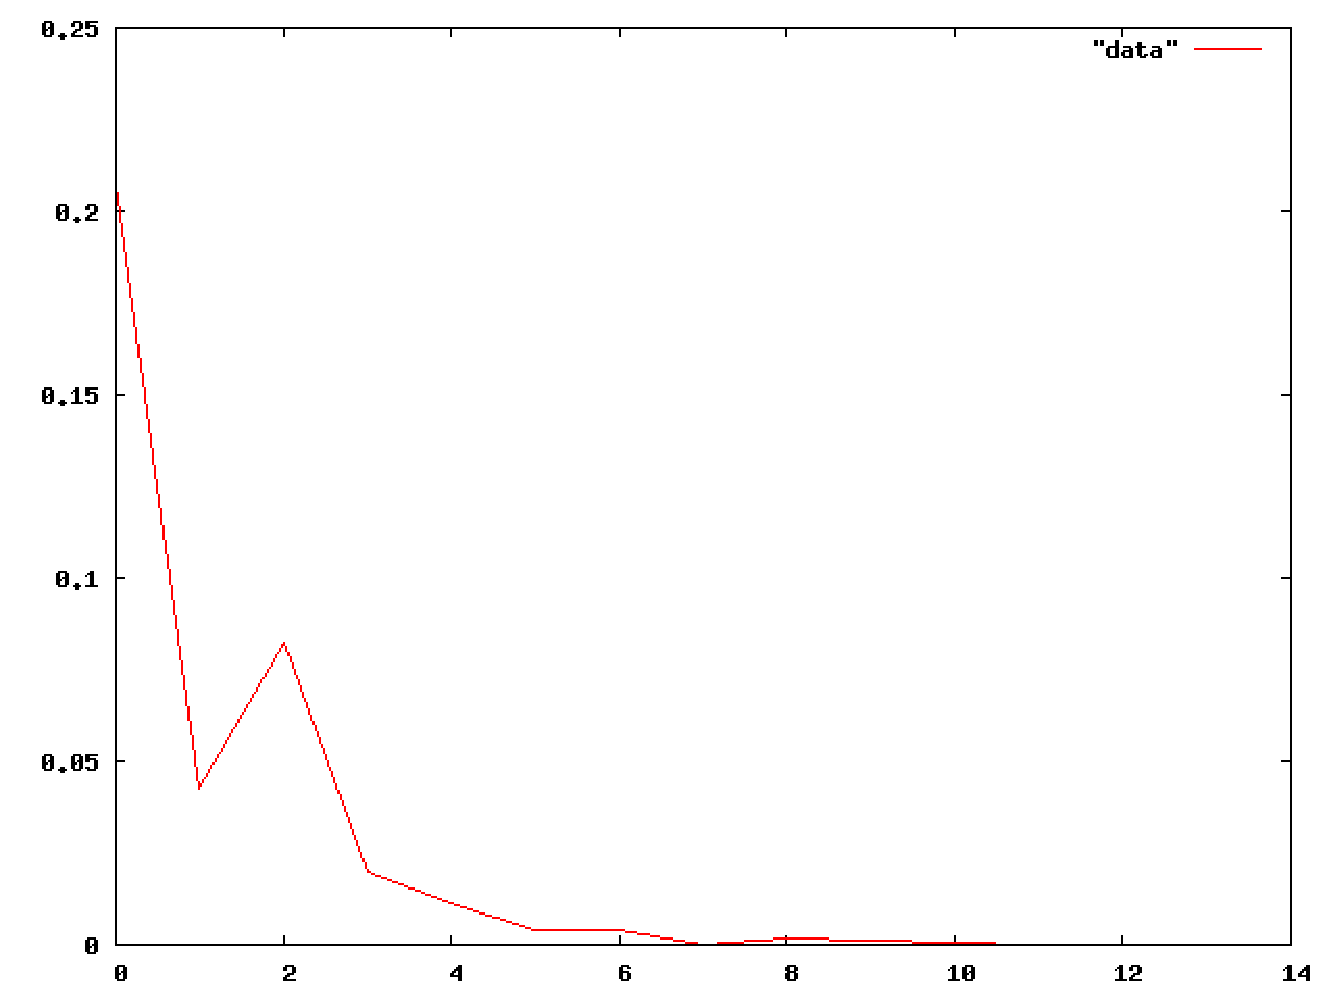
\includegraphics[width=0.7\textwidth]{./images/grafico}
\end{figure}


%%%%%%%%%%%%%%%%%%%%%

\documentclass[12pt,twoside]{article}
\usepackage{amsmath,amssymb}
\usepackage{a4wide}
\begin{document}
Here you find a simple set of codes for the problem: find $\mathbf{x}$ such that
\[
\mathbf{F}(\mathbf{x})=\mathbf{0}
\]
for a $F:\mathbb{R}^n\to\mathbb{R}^n$ (which we assume to be at least Lipschitz continuous).

The set of codes include a class to store non linear systems, a class thet implements Newton method and another for a genetic fixed point iteration.
\section{The class for non linear systems}

\section{The methods implemented}
\subsection{Newton Method}
We indicate with $\boldsymbol{J}(\mathbf{x})$ the Jacobian (Frechet derivative) of $\mathbf{F}$ at $\mathbf{x}$. The algorithm implements a simple backtraching
based on Armijo rule with constant reduction of the step $\lambda$.

Let $\mathbf{x}$ be given, together with a small positive number $\sigma$ and
$\gamma\in (0,1)$
\begin{enumerate}
\item Compute $\mathbf{d}$ by solving
$
\boldsymbol{J}(\mathbf{x})\mathbf{d}=-\mathbf{F}(\mathbf{x}).
$
\item $\lambda=1$.
\item Until $\Vert\mathbf{F}(\mathbf{x}+\lambda\mathbf{d})\Vert< (1-\lambda\sigma)\Vert \mathbf{F}(\mathbf{x}\Vert$ set $\lambda\leftarrow
\gamma\lambda$
\item Set $\mathbf{x}\leftarrow\mathbf{x}+\lambda\mathbf{d}$
\item Check for convergence.
\end{enumerate}
Convergence test is made by checking the residual $\mathbf{F}(\mathbf{x})$, the
step length $\Vert \mathbf{d}\Vert$ and fixing a maximum number of iterations.

Step 3 implements Armijo rule for sufficient decrease of $\Vert\mathbf{F}\Vert$.

\section{Notes}
The architecture of this code can be bettered. First of all one can generalize the class fixed point to accept any iteration function $\boldsymbol{\Phi}(\mathbf{x})$ and implements
\[
\mathbf{x}_{k+1}=\boldsymbol{\Phi}(\mathbf{x}_k), \quad k=1,\ldots
\]
for a given $\mathbf{x}_0$.

In this respect Newton method is just a  particular fixed point iteration with iteration function
\[
\boldsymbol{\Phi}_N(\mathbf{x})=\mathbf{x}-\boldsymbol{J}^{-1}(\mathbf{x})\mathbf{F}(\mathbf{x})
\]

However Newton method can be seen as a particular \emph{line search method}. So one may think to create an abstract class (or a template) for generic line search methods and specialise it for different type of algorithms, using for instance a stategy pattern via policies. Algoritms may include gradient, conjugate gradient (in different forms), Broyden etc etc. It may also implement different backtracking strategies (armijo, Wolfe....) 
All algoritms of the form
\begin{itemize}
\item Compute a descent direction $\mathbf{d_k}$
\item Compute the step $\mathbf{\alpha}_k$ according to a backtracking strategy
\item Update $\mathbf{x}_{k+1}=\mathbf{x}_k+\alpha_k\mathbf{d}_k$.
\end{itemize}
\end{document}
%%% Local Variables:
%%% mode: latex
%%% TeX-master: t
%%% End:


\bibliographystyle{siam}
\bibliography{../common/bibliography}

\end{document}
